\chapter{Minecraft as a Simulation Environment for MicroPsi 2}
The objective of this project is to build and test an interface in between MicroPsi and Minecraft, so that a Minecraft world (e.g. server) can be used as a simulation environment for the MicroPsi 2 Framework, which will act as an artificial player.

The modular architecture of MicroPsi 2 allows it to add new simulation environments (or worlds, as they are called in MicroPsi) fairly easily. To communicate with a MicroPsi node net, a world needs an interface which is called world adapter. The world adapter has to define data sources and targets. It fills the sources with data from the world and writes the targets to the world. The node net does the opposite: it reads from the sources and writes into the targets. This enables a feedback loop in between the world and the node net.

Furthermore, the world adapter provides a step function, that advances the world and is called by the MicroPsi world runner frequently.

Looking at the Minecraft side, communication with a Minecraft Server typically requires a constant flow of data packets going in and out. Most third party clients, including Bots, facilitate own event loops.

To add a ``Minecraft'' world to MicroPsi, the demands of both sides have to be met.

    \section{Using Spock as the interface in between MicroPsi and a Minecraft server}
The calculation of the simulation environment, does not take place in MicroPsi itself, but on a regular Minecraft Server. Instead, Spock is integrated into MicroPsi and represents the simulation world towards it. Spock communicates with the Minecraft server via the Client-Server-Protocol and provides data that can be used as data sources for the world adapter and translates the data from the data targets to actions in the simulation environment. That way, to MicroPsi it looks like Spock is the simulation environment itself, where in fact it's the interface to game world server.

The original event loop of the bot framework had to be dissolved and rebuilt as the step function of the MicroPsi world. The event loop and handling of spock had to be slightly modified to work with MicroPsi. It should be noted, that the frequency in which the framework steps the bot has to be at least chosen high enough, so that it is able to send the necessary keep-alive-signals, to not get kicked from the server.

Eventually, useful data sources had to be picked and generated and a system of data targets and their translation to actual actions had to be implemented. In most cases, performing actions means to let spock send a specific set of packets to the Minecraft server.

\paragraph{Data Targets and sources}

... diamonds ...


    \section{The Visualisation component}
That being said, the other important part of this project is the visualisation component. Inside the world adapter's step function, the visualisation module is called to generate a 3D model of the Minecraft world and the agent within. There are two main reasons for this. The first reason is, that the agent's behaviour within the simulation environment is supposed to be visually monitored from the MicroPsi web interface --- in a both effective and pleasurable manor. The second reason is, that the image data is supposed to be processed by the node net as a data source itself in the future.

The visualisation component reads from Spock's internal gameworld representation to generate the 3D model. This means, that from pure Minecraft world data a 3D-visualisation has to be generated from within the MicroPsi Python Code. It should contain a perspective that gives a good overview over the bots environment to forward to the web interface, as well as a the agent's first person perspective, to function as a data source in the future.  

The visualisation is in it's heart based on ``Minecraft'' by Michael Fogleman.

Specifically, the representation of the chunk, the agent is located in, is fetched and for each solid cube in this chunk, a corresponding cube is rendered within the visualisation using Pyglet's OpenGL abstraction. Each block gets textures according to it's type. The implemented format for the textures is compatible to the widely available Minecraft texture packs. That way, the visualisation's look can be changed completely within seconds. The resulting images are exported as JPEG files. Then, they are displayed in the web interface. A refresh rate of six or more images per second creates the impression of a video stream.

Similar to spock, ``Minecraft'' by Michael Fogleman used it's own event-loop and -handling. Again, the event loop had to be disassembled and rebuilt as a part of the world adapter's step function, which advances the visualisation with every step.

Viewing the resulting software as a whole, several modules have been added to the architecture: the Minecraft world adapter, the Spock bot (facilitating communication with the Minecraft Server) and the visualisation component. (see figure \ref{uml_mc})

\begin{figure}[h]
  \centering
    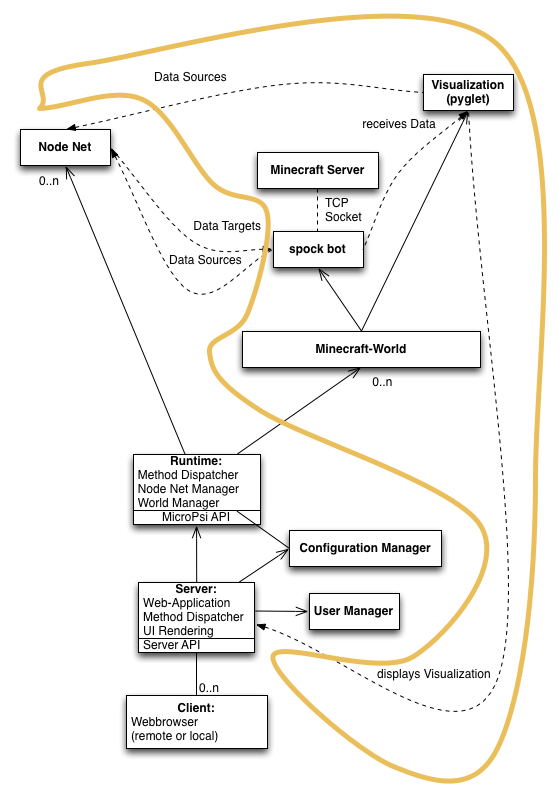
\includegraphics[width=10cm]{graphics/UML_MicroPsi_mit_spock_und_rahmen}
  \caption{The new architecture of MicroPsi with the Minecraft interface. New modules are framed orange.}
  \label{uml_mc}
\end{figure}

%TODO ... illustration of the event loop ...

% TODO je nach Größe des Kapitels, das hier vielleicht eine Ebene höher ziehen (versuche dich hier erstmal nur auf die fertige Lösung zu konzentrieren und warum du dich dafür entschieden hast. Es ist nicht interessant, was du sonst alles ausprobiert hast, außer dass du konkret angibst, warum du dich für die jetztige Implementierung im Vergleich zu anderen entschieden hast)

    \section{Case Study}
As a proof of concept, the functionality of this project has been tested with a simple Braitenberg-vehicle experiment.